\documentclass[11pt]{article}

% This first part of the file is called the PREAMBLE. It includes
% customizations and command definitions. The preamble is everything
% between \documentclass and \begin{document}.

\usepackage[margin=1in]{geometry}  % set the margins to 1in on all sides

\usepackage{graphicx}              % to include figures
\usepackage{amsmath}               % great math stuff
\usepackage{amsfonts}              % for blackboard bold, etc
\usepackage{amsthm}                % better theorem environments

\usepackage{dcolumn}
\usepackage{dsfont}
\usepackage{array}
\usepackage{booktabs}
\usepackage{soul}
\usepackage{mathrsfs}
\usepackage{enumerate}
\usepackage{multicol}
\usepackage[makeroom]{cancel}
\usepackage{xcolor}
\usepackage{tikz}
\usepackage{pdfpages}

% various theorems, numbered by section

\newtheorem{thm}{Theorem}[section]
\newtheorem{lem}[thm]{Lemma}
\newtheorem{prop}[thm]{Proposition}
\newtheorem{cor}[thm]{Corollary}
\newtheorem{conj}[thm]{Conjecture}
\newtheorem{exer}[thm]{Exercise}

\DeclareMathOperator{\id}{id}

\newcommand{\EE}{\mathbb{E}}
\newcommand{\ff}{\boldsymbol{f}}
\newcommand{\Hl}{\boldsymbol{H}_\lambda}
\newcommand{\II}{\boldsymbol{I}}
\newcommand{\ee}{\boldsymbol{e}}
\newcommand{\yy}{\boldsymbol{y}}
\newcommand{\bd}[1]{\mathbf{#1}}  % for bolding symbols
\newcommand{\RR}{\mathbb{R}}      % for Real numbers
\newcommand{\ZZ}{\mathbb{Z}}      % for Integers
\newcommand{\col}[1]{\left[\begin{matrix} #1 \end{matrix} \right]}
\newcommand{\comb}[2]{\binom{#1^2 + #2^2}{#1+#2}}
\newcommand{\overfrac}[2]{\genfrac{}{}{0pt}{}{#1}{#2}}

\renewcommand{\thesubsection}{\thesection.\alph{subsection}}

\everymath{\displaystyle}

\setlength\parindent{0pt}

\usepackage{setspace}

\begin{document}
\begin{multicols}{2}
  \phantom{hello}\vspace{0.01\baselineskip}
  \phantom{hello}\vspace{0.01\baselineskip}
  {\large Assignment 6}\\
  \begin{flushright}
    Mikhail Gaerlan (914437675)\\
    9 June 2017\\
    STA 243 Lee
  \end{flushright}
\end{multicols}
\vspace{-2.3\baselineskip}

\hrulefill

\section{}

\subsection{}

\begin{eqnarray*}
  F\left(x\right)&=&P\left(\hat{\theta}<x\right)\\
                 &=&P\left(\textrm{max}\left(X_1,\ldots,X_n\right)\right)\\
                 &=&P\left(\left(X_1<x\right)\cup\cdots\cup\left(X_n<x\right)\right)\\
                 &=&P\left(X_1<x\right)+\cdots+P\left(X_n<x\right)\\
                 &=&\left\{\begin{array}{ccl}
                             0&,&x<0\\
                             \left(\frac{x}{\theta}\right)^n&,&0\leq x\leq \theta\\
                             1&,&\theta<x
                           \end{array}
                                 \right.\\
  f\left(x\right)&=&\frac{d}{dx}\,F\left(x\right)\\
                 &=&\left\{\begin{array}{ccl}
                             0&,&x<0\\
                             \frac{n}{\theta}\left(\frac{x}{\theta}\right)^{n-1}&,&0\leq x\leq \theta\\
                             0&,&\theta<x
                           \end{array}
                                 \right.\\
\end{eqnarray*}

\subsection{}

\begin{eqnarray*}
  \textrm{Var}_{F_\theta}\left(\hat{\theta}\right)&=&\int_0^\theta x^2\frac{n}{\theta}\left(\frac{x}{\theta}\right)^{n-1}dx-\left(\int_0^\theta x\frac{n}{\theta}\left(\frac{x}{\theta}\right)^{n-1}dx\right)^2\\
                                                  &=&\left.\frac{n}{n+2}\frac{x^{n+2}}{\theta^n}\right|_{x=0}^{x=\theta}-\left(\left.\frac{n}{n+1}\frac{x^{n+1}}{\theta^n}\right|_{x=0}^{x=\theta}\right)^2\\
                                                  &=&\frac{n}{n+2}\theta^2-\left(\frac{n}{n+1}\theta\right)^2\\
                                                  &=&\theta^2\frac{n}{\left(n+1\right)^2\left(n+2\right)}
\end{eqnarray*}

\subsection{}

\begin{eqnarray*}
  \textrm{Var}_{F_\theta}\left(\hat{\theta}\right)&=&\theta^2\frac{n}{\left(n+1\right)^2\left(n+2\right)}\\
                                                  &\approx&0.003327123\\
  \textrm{Var}_{F_\theta}\left(\hat{\theta}_B\right)&\approx&0.003458246
\end{eqnarray*}

\subsection{}

\begin{eqnarray*}
  \textrm{Var}_{F_\theta}\left(\hat{\theta}_B\right)&\approx&0.004655322
\end{eqnarray*}

\subsection{}

\begin{table*}[h]
  \begin{center}
    \renewcommand{\arraystretch}{1.5}
    \begin{tabular}{| >{\centering\arraybackslash}m{3in} |  >{\centering\arraybackslash}m{3in} |}
      \hline
      Parametric Bootstrap
      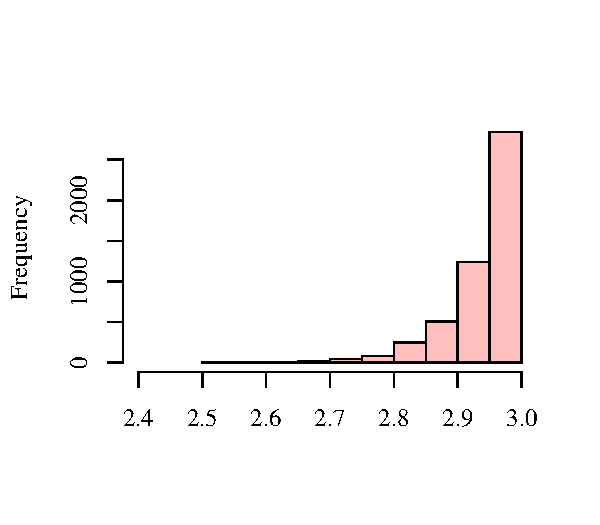
\includegraphics[width=1\linewidth,height=0.3\textheight]{Graphs/parametricboot}&
      Nonparametric Bootstrap
      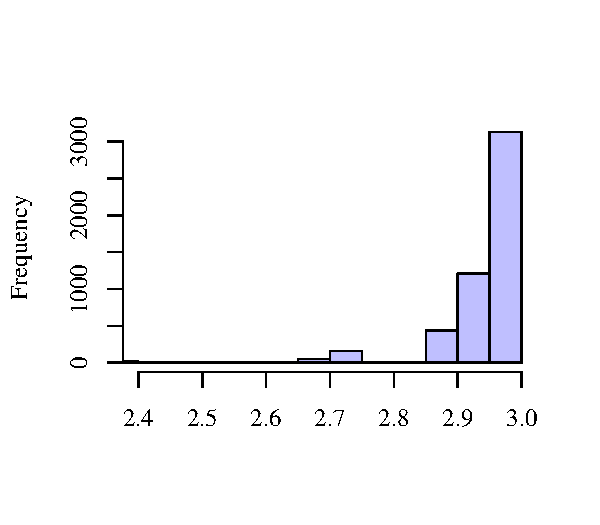
\includegraphics[width=1\linewidth,height=0.3\textheight]{Graphs/nonparametricboot}\\\hline
    \end{tabular}
  \end{center}
\end{table*}

\subsection{}

The distribution seems to matches up very well to the histograms in Part 1.e.
\begin{figure}[h!]
\begin{center}
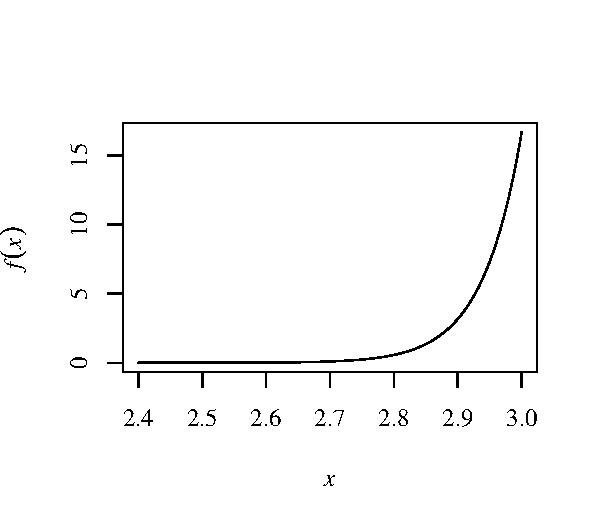
\includegraphics[height=0.4\textheight,width=0.6\linewidth]{Graphs/distribution}
\end{center}
\end{figure}

\section{}

\subsection{}

\begin{table*}[h]
  \begin{center}
    \renewcommand{\arraystretch}{1.5}
    \begin{tabular}{| >{\centering\arraybackslash}m{3in} |  >{\centering\arraybackslash}m{3in} |}
      \hline
      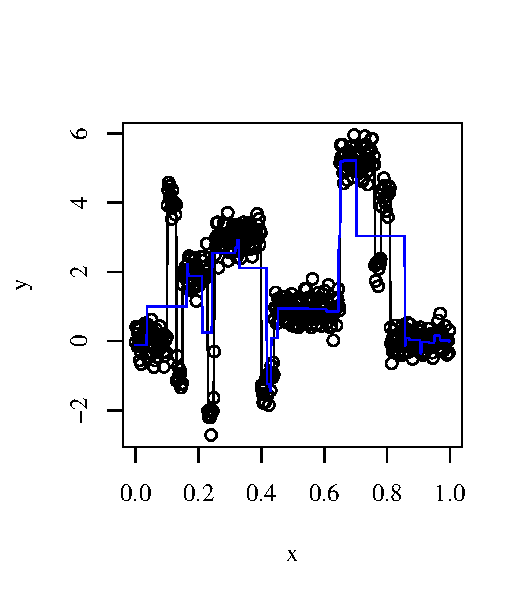
\includegraphics[width=1\linewidth,height=0.3\textheight]{Graphs/fitted}&
      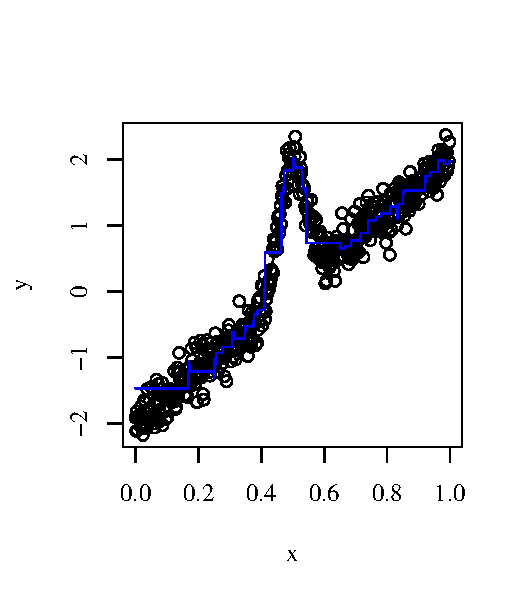
\includegraphics[width=1\linewidth,height=0.3\textheight]{Graphs/other}\\\hline
    \end{tabular}
  \end{center}
\end{table*}

\subsection{}

\begin{table*}[h]
  \begin{center}
    \renewcommand{\arraystretch}{1.5}
    \begin{tabular}{| >{\centering\arraybackslash}m{3in} |  >{\centering\arraybackslash}m{3in} |}
      \hline
      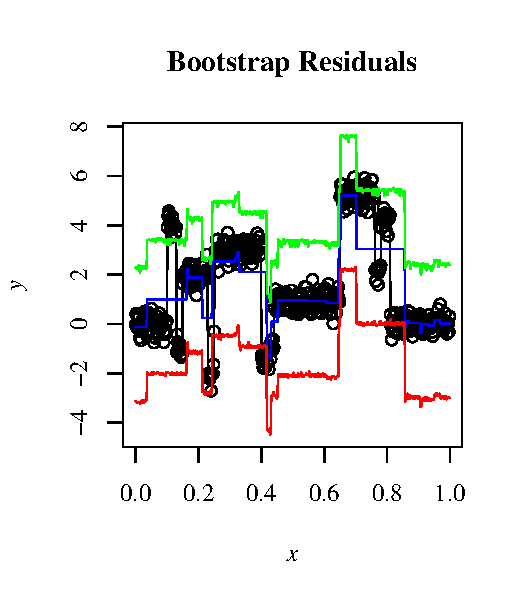
\includegraphics[width=1\linewidth,height=0.3\textheight]{Graphs/confidenceresid1}&
      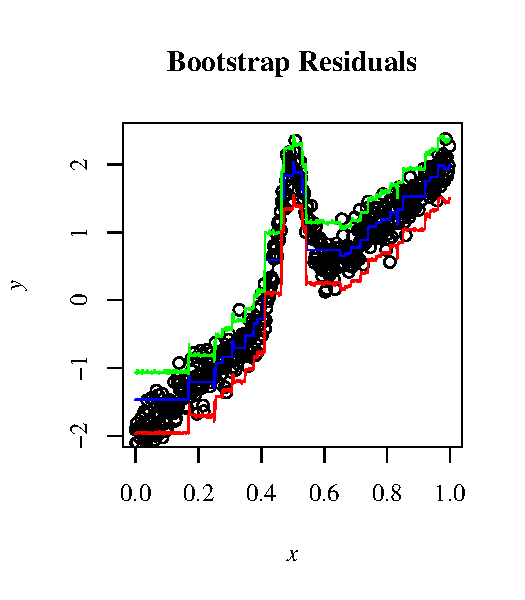
\includegraphics[width=1\linewidth,height=0.3\textheight]{Graphs/confidenceresid2}\\\hline
    \end{tabular}
  \end{center}
\end{table*}

\subsection{}

A confidence interval for the first jump, for example, could be found by finding $B$ models then finding the mean of the standard deviation of the first jump. Then the 95\% confidence interval would be the mean plus or minus two standard deviations.

\section{}

\subsection{}

\subsection{}

\subsection{}

\end{document}